\documentclass{article}

\usepackage[english]{babel}

\usepackage[letterpaper,top=2cm,bottom=2cm,left=3cm,right=3cm,marginparwidth=1.75cm]{geometry}

% Useful packages
\usepackage{graphicx}

\begin{document}

\section{Framework Design}

\subsection{Design Approach}

We designed a lightweight single-agent coding harness built on Microsoft's AutoGen AgentChat. The framework aims to automate the generation, compilation, and iterative repair of PLC (Programmable Logic Controller) Structured Text (ST) programs. Rather than adopting a multi-agent architecture, we decided to use a single agent, \textit{CodeGeneratorAgent}, combined with a custom orchestration layer, \textit{PLCHarness}. This design separates LLM-based code generation from deterministic compilation, reducing unnecessary model calls and providing a consistent execution workflow across different LLMs.

\subsection{System Architecture}

The system consists of three main components:

\begin{itemize}
\item \textbf{\textit{CodeGeneratorAgent}}: An AutoGen AssitantAgent that generates ST code from natural-language requirements and repairs code using feedback provided by the compiler.
\item \textbf{\textit{PLCHarness}}: A self-developed orchestration layer responsible for context management, task execution, compilation, iterative repair, and termination logic.
\item \textbf{CODESYS Compilation Service}: An external HTTP service that compiles generated ST code in CODESYS and returns structured compilation results.
\end{itemize}

The framework follows a predefined generation–compilation–repair workflow, consisting of the following steps:

\begin{enumerate}

\item \textbf{Agent Initialization}: The system initializes \textit{CodeGeneratorAgent} with a predefined system message specifying its role, responsibilities, and expected behavior.

\item \textbf{Task Execution}: The harness provides the natural-language PLC programming task to the agent, which generates ST code based on the given requirements.

\item \textbf{Compilation}: The harness automatically invokes the compilation tool, which submits the generated ST code to the CODESYS compiler and returns structured compilation results, including any detected errors.

\item \textbf{Successful Compilation}: If compilation succeeds, the harness terminates the iterative process and records the generated code and execution results.

\item \textbf{Iterative Repair}: If compilation fails and the maximum number of repair attempts has not been reached, the harness forwards the compiler feedback to the agent, which generates a revised implementation. The compilation and repair cycle continues until compilation succeeds or a termination condition is met.

\end{enumerate}

\begin{figure}
\centering
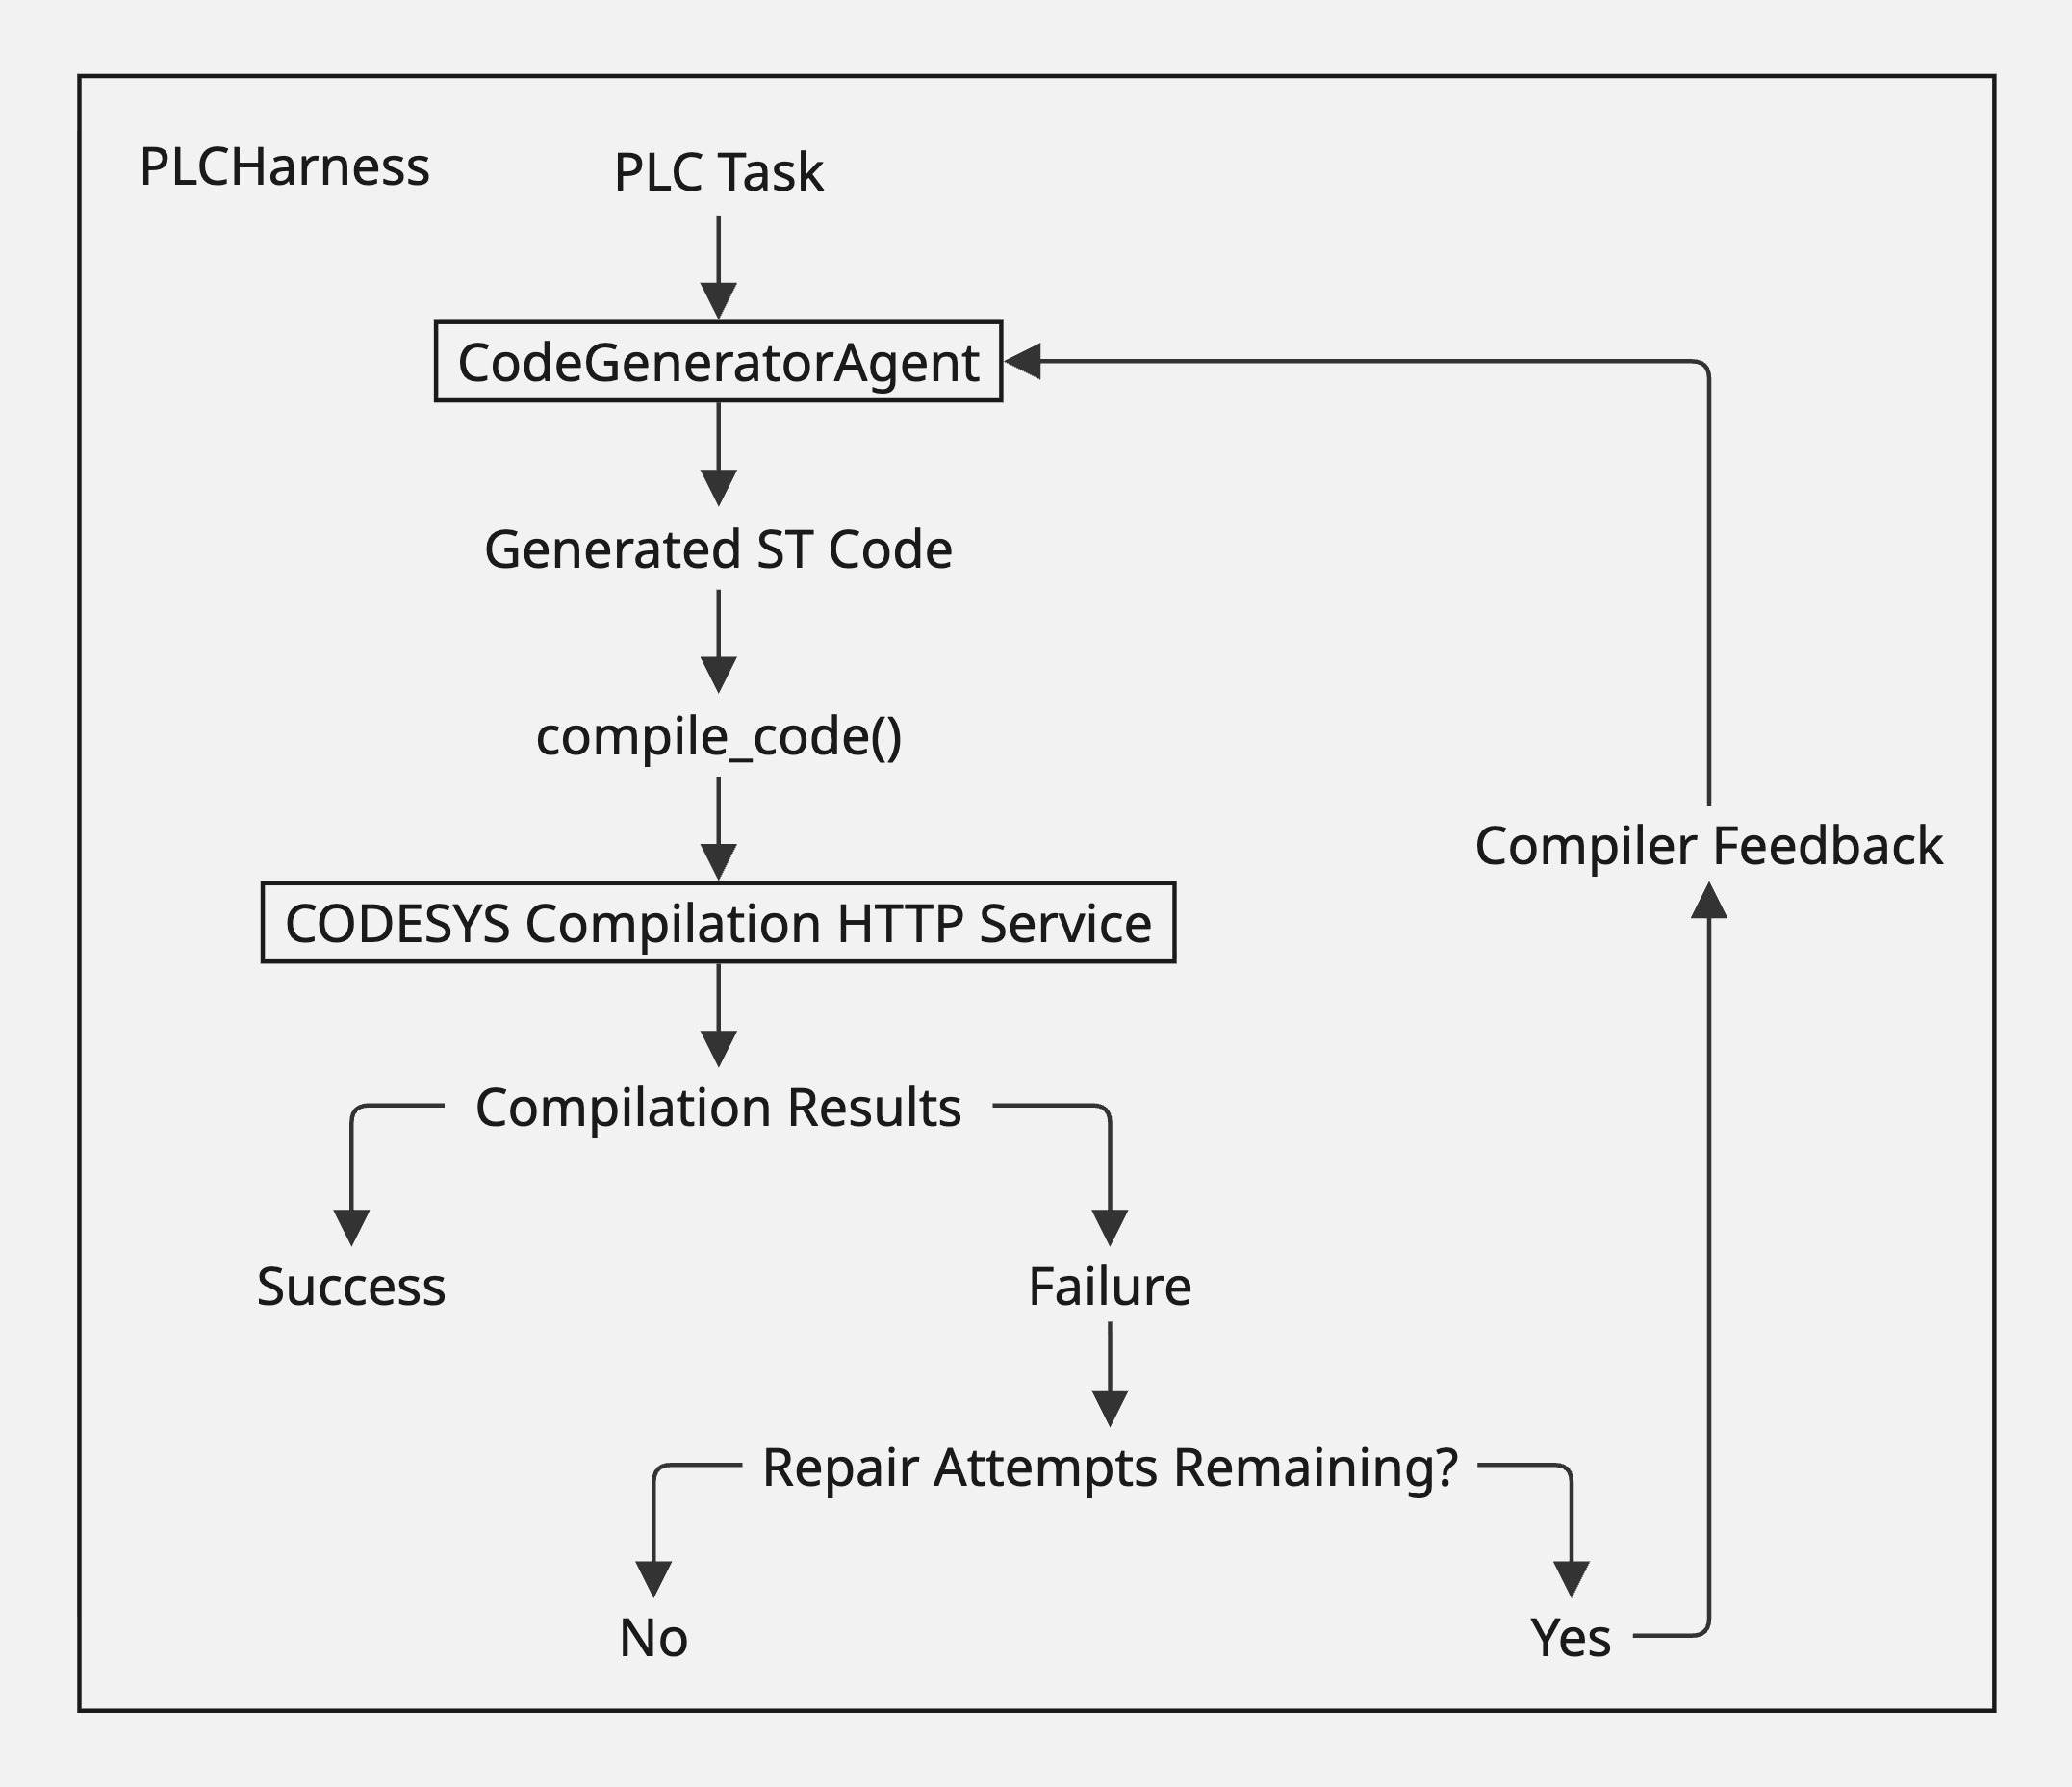
\includegraphics[width=0.75\linewidth]{workflow.jpg}
\caption{\label{fig:workflow}Execution workflow of the PLCGen generation-compilation-repair process.}
\end{figure}


\subsection{Harness Design Principles}

\subsubsection{Task Organization}

Task organization is implemented at two levels. At the dataset level, the main program loads the problems from a structured JSON file, assigns unique task identifiers, and executes them sequentially. At the individual task level, the \textit{PLCHarness} class coordinates code generation, compilation, and repair according to the predefined workflow. In this way, we allow independent task execution while maintaining a consistent procedure across all problems.

\subsubsection{Context Management}

The stateful nature of AutoGen's AssistantAgent allows it to retain task requirements, previously generated code, and compiler feedback across repair iterations by maintaining the conversation history. This reduces redundant input and enables the agent to use information from previous attempts when refining its code. To ensure independence between PLC programming problems and prevent context contamination, the agent's conversation state is reset before each new task.

\subsubsection{Tool Invocation}

The compilation tool is automatically invoked after each code-generation attempt, ensuring that every generated code is checked for compilation errors. Rather than allowing the LLM to decide when to invoke it, the harness follows a deterministic workflow, reducing unnecessary LLM calls and ensuring consistent execution across different models.

\subsubsection{Compilation and Repair}

The compilation tool processes the results returned by the CODESYS HTTP service, distinguishing compilation failures from tool execution errors. When compilation fails, the harness extracts the relevant compiler error messages and forwards them to \textit{CodeGeneratorAgent}. Using the retained task context and compiler feedback, the agent generates a revised ST implementation, which is subsequently submitted for another compilation attempt. This process continues until compilation succeeds or a termination condition is reached. Tool execution errors are handled separately to avoid unnecessary repair attempts when the compilation service encounters an unexpected failure.

\subsubsection{Termination Conditions}

The generation–compilation–repair loop terminates when compilation succeeds or the maximum number of repair attempts is reached. Additional termination conditions include empty or repeated code generation, compilation tool failures, and missing compiler feedback. These conditions prevent redundant iterations, unnecessary API calls, and potentially unproductive repair loops.

\subsection{Implementation}

The framework is implemented across four main Python files, each responsible for a specific component of the system:

\begin{itemize}
\item \textit{common.py}: Provides shared utility methods for configuration management, LLM client initialization, command-line argument parsing, output directory creation, and result saving.
\item \textit{main.py}: Serves as the main entry point, handling system initialization, task loading, sequential task execution, and the collection of experimental results.
\item \textit{agent.py}: Defines \textit{CodeGeneratorAgent} and implements the custom \textit{PLCHarness}, which coordinates the generation–compilation–repair workflow described in the previous sections.
\item \textit{tools.py}: Implements the \textit{compile\_code()} function, which communicates with the CODESYS HTTP service to submit generated ST code and retrieve structured compilation results and error messages.
\end{itemize}

\end{document}
